\documentclass[12pt,oneside]{article}

%%%%%%%%%%%%%%%%%%%%%%%%%%%%
%%   Zusaetzliche Pakete  %%
%%%%%%%%%%%%%%%%%%%%%%%%%%%%
\usepackage{acronym}
\usepackage{enumerate}
\usepackage{a4wide}
\usepackage{fancyhdr}
\usepackage[pdftex]{graphicx}
\usepackage{palatino}
\usepackage{blindtext}
\usepackage{multirow}
\usepackage[ruled,longend]{algorithm2e}
\usepackage{float}
\usepackage{amsmath}
\usepackage{amssymb}
\usepackage{listings}
\usepackage[numbib]{tocbibind}

%folgende Zeile auskommentieren für englische Arbeiten
\usepackage[ngerman]{babel}

%folgende zeile auskommentieren und die darunter verwenden, um die link-border zu verbergen
%\usepackage[bookmarks]{hyperref}
\usepackage[bookmarks,hidelinks]{hyperref}
\usepackage[T1]{fontenc}
\usepackage[utf8]{inputenc}
\usepackage[a-1b]{pdfx}
\usepackage[justification=centering]{caption}
%\usepackage[style=unsrt,natbib=true,backend=biber]{biblatex}
\usepackage{csquotes}
\usepackage{url}
%\usepackage{subfigure}
\usepackage[utf8]{inputenc}
\usepackage[T1]{fontenc}
% Layout corrections (Schusterjungen)
\clubpenalty = 10000 
% Layout corrections (Hurenkinder) 
\widowpenalty = 10000 
\displaywidowpenalty = 10000

% Figures
\usepackage{caption}
\usepackage[hypcap=true,labelformat=simple]{subcaption}
\renewcommand{\thesubfigure}{(\alph{subfigure})}

% Tables
\usepackage{booktabs} 

% Newcommand TODO (red in text)
\newcommand{\todo}[1]{\textcolor{red}{TODO: #1}}

% Newcommand TODOM (red at border)
\newcommand{\todom}[1]{\marginpar{\parbox{1.5cm}{\textcolor{red}{TODO:\\ #1}}}}

% Format für dd.mm.yyy format
\newcommand{\todayddmmyyyy}{%
  \ifnum\day<10 0\fi\the\day.%
  \ifnum\month<10 0\fi\the\month.%
  \the\year}



%%%%%%%%%%%%%%%%%%%%%%%%%%%%%%
%% Definition der Kopfzeile %%
%%%%%%%%%%%%%%%%%%%%%%%%%%%%%%

\pagestyle{fancy}
\fancyhf{}
\cfoot{\thepage}
\setlength{\headheight}{16pt}

%%%%%%%%%%%%%%%%%%%%%%%%%%%%%%%%%%%%%%%%%%%%%%%%%%%%%
%%  Definition des Deckblattes und der Titelseite  %%
%%%%%%%%%%%%%%%%%%%%%%%%%%%%%%%%%%%%%%%%%%%%%%%%%%%%%

\newcommand{\HSFTitle}[8]{

  \thispagestyle{empty}
\begin{center}
    
\includegraphics[width=0.9\textwidth]{logo_new_2.png} \\
    \vspace*{\stretch{1}}
    \end{center}

  %\vspace*{\stretch{1}}
  {\parindent0cm
  \rule{\linewidth}{.7ex}}
  \begin{center}
    \vspace*{\stretch{1}}
    \sffamily\bfseries\Huge
    #1\\
    \vspace*{\stretch{1}}
    \sffamily\bfseries\large
    #3
    \vspace*{\stretch{1}}
  \end{center}
  \rule{\linewidth}{.7ex}

  \vspace*{\stretch{2}}
  \begin{center}
    \Large #2 am #5 der HS Fulda \\
    \vspace*{\stretch{1}}

    \large Matrikelnummer:  #4 \\[1mm]
    \large Projektcode: Automatentyp Nr. 0 - Musikautomat (Jukebox) \\[1mm]
    \large Erstbegutachtung:  #7 \\[1mm]

    \vspace*{\stretch{1}}
    \large Eingereicht am #6
  \end{center}
}


%%%%%%%%%%%%%%%%%%%%%%%%%%%%
%%  Beginn des Dokuments  %%
%%%%%%%%%%%%%%%%%%%%%%%%%%%%

\begin{document}

  \HSFTitle
      {Spezifikation eines Musikautomaten (Jukebox) mit UML}       % Titel der Arbeit
      {Prüfungsteil 1 (Software Engineering)} % Typ der Arbeit
      {Luca M. Schmidt}          % Vor- und Nachname der Autor*in
      {1540963}
      {Fachbereich AI}  % Name des FBs
      {\todayddmmyyyy}        % Tag der Abgabe
      {Prof. Dr. Cathrin Möller}     % Name der Erstgutachter*in

  \clearpage

\lhead{}
\pagenumbering{Roman}
    \setcounter{page}{1}

%\addcontentsline{toc}{section}{\listfigurename}
\tableofcontents
\listoffigures
%\addcontentsline{toc}{section}{\listtablename}
\clearpage


%%%%%%%%%%%%%%%%%%%%%%%%%%%%
%%  Einstellungen  %%
%%%%%%%%%%%%%%%%%%%%%%%%%%%%
\cleardoublepage
\pagenumbering{arabic}
    \setcounter{page}{1}
\lhead{\nouppercase{\leftmark}}

%%%%%%%%%%%%%%%%%%%%%%%%%%%%
%%  Hauptteil  %%
%%%%%%%%%%%%%%%%%%%%%%%%%%%%

\section{Funktionsbeschreibung des Musikautomaten} \label{sec:funktionsbeschreibung}
Der Musikautomat ist ein moderner, coin-betriebener Automat für öffentliche Bereiche. Nutzer werfen einen speziellen Coin ein, um Zugang zu einem digitalen Musikkatalog zu erhalten. Die Bedienung erfolgt über ein Touchscreen zur Navigation durch Kategorien (Genre, Künstler, Charts) oder eine Suchfunktion.\\
Nach der Songauswahl werden Titel einer Warteschlange (Queue) hinzugefügt und in der Reihenfolge abgespielt. Das System zeigt während der Wiedergabe Metadaten wie Interpret und Titel an. Steuerungsoptionen wie Pause oder Skip sind bewusst deaktiviert, um Missbrauch zu vermeiden.\\
Der Automat ist permanent mit einem externem Gerät des Besitzers vernetzt. Diese ermöglicht die Fernaktualisierung des Musikkatalogs, Konfiguration von Lautstärke und Betriebszeiten sowie die Sammlung von Nutzungsstatistiken für Lizenzabrechnung. Wartung erfolgt sowohl digital (Software-Updates, Katalog-Synchronisation) als auch physisch (Reinigung, Coin-Entleerung, Hardware-Reparaturen).

\begin{figure}[H]
    \centering
    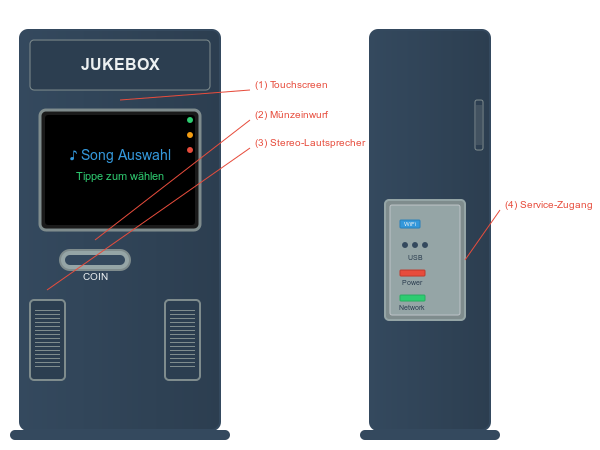
\includegraphics[width=\textwidth]{images/jukebox_technical_sketch.png}
    \caption{Technische Skizze eines modernen Musikautomaten}
    \label{fig:jukebox_skizze}
\end{figure}
\noindent
Die primäre Nutzerinteraktion konzentriert sich auf das zentrale Touchscreen-Display (1), das sowohl zur Navigation im Musikkatalog als auch zur Anzeige von Systeminformationen dient. Der Coin-Einwurfmechanismus (2) ist mit einem integrierten Validierungssystem ausgestattet, das gefälschte oder beschädigte Coins automatisch erkennt und zurückweist. Die Audio-Ausgabe erfolgt über professionelle Stereo-Lautsprecher (3), die für den Dauerbetrieb in öffentlichen Umgebungen optimiert sind. Der Service-Zugang (4) ist durch ein Sicherheitsschloss geschützt und ermöglicht autorisiertem Personal den Zugriff auf interne Komponenten für Wartungs- und Reparaturarbeiten.

\section{UML-Diagramme} \label{sec:uml_diagramme}
Die folgenden beiden UML-Diagramme zeigen verschiedene Aspekte des Musikautomaten und ergänzen sich in ihrer Darstellung.

\subsection{Aktivitätsdiagramm: Songauswahl und -wiedergabe}
Das Aktivitätsdiagramm in Abbildung \ref{fig:activity_diagram} stellt den typischen Nutzungsprozess vom Coin-Einwurf bis zur Songwiedergabe dar.

\begin{figure}[H]
    \centering
    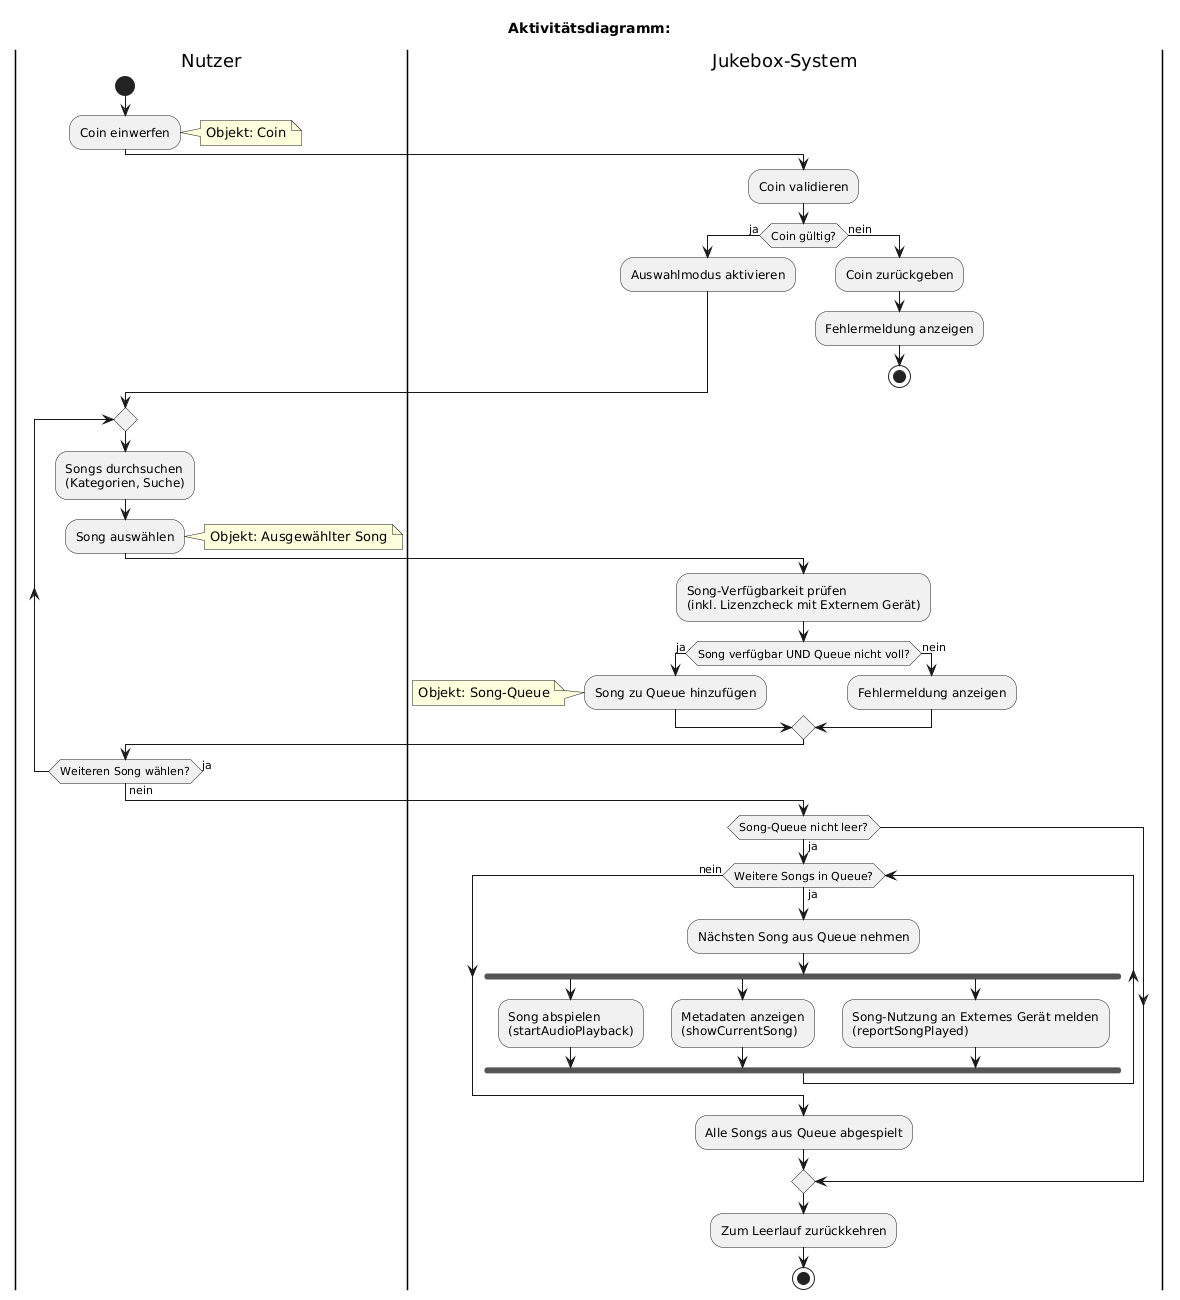
\includegraphics[width=\textwidth]{images/activity_diagram.png}
    \caption{Aktivitätsdiagramm: Songauswahl und -wiedergabe mit Nutzer-System-Interaktionen}
    \label{fig:activity_diagram}
\end{figure}
\noindent
\textbf{Ablauf:} Der Nutzer wirft einen Coin ein, das System validiert ihn und aktiviert bei Gültigkeit den Auswahlmodus. Nach der Songauswahl prüft das System die Verfügbarkeit und fügt verfügbare Songs zur Queue hinzu. Parallele Wiedergabe-Aktivitäten umfassen Abspielen, Metadaten-Anzeige und Zentrale-Kommunikation.

\subsection{Sequenzdiagramm: Songwiedergabe und Interaktion mit externem Gerät}
Das Sequenzdiagramm in Abbildung \ref{fig:sequence_diagram} fokussiert sich auf die zeitliche Choreographie der Nachrichten und Interaktionen zwischen den verschiedenen Systemkomponenten während des kritischen Prozesses der Songwiedergabe. Besondere Aufmerksamkeit gilt dabei der Kommunikation mit dem externem Gerät des Besitzers, welches für Lizenzmanagement, Nutzungsstatistiken und Systemüberwachung verwendet wird.

\begin{figure}[H]
    \centering
    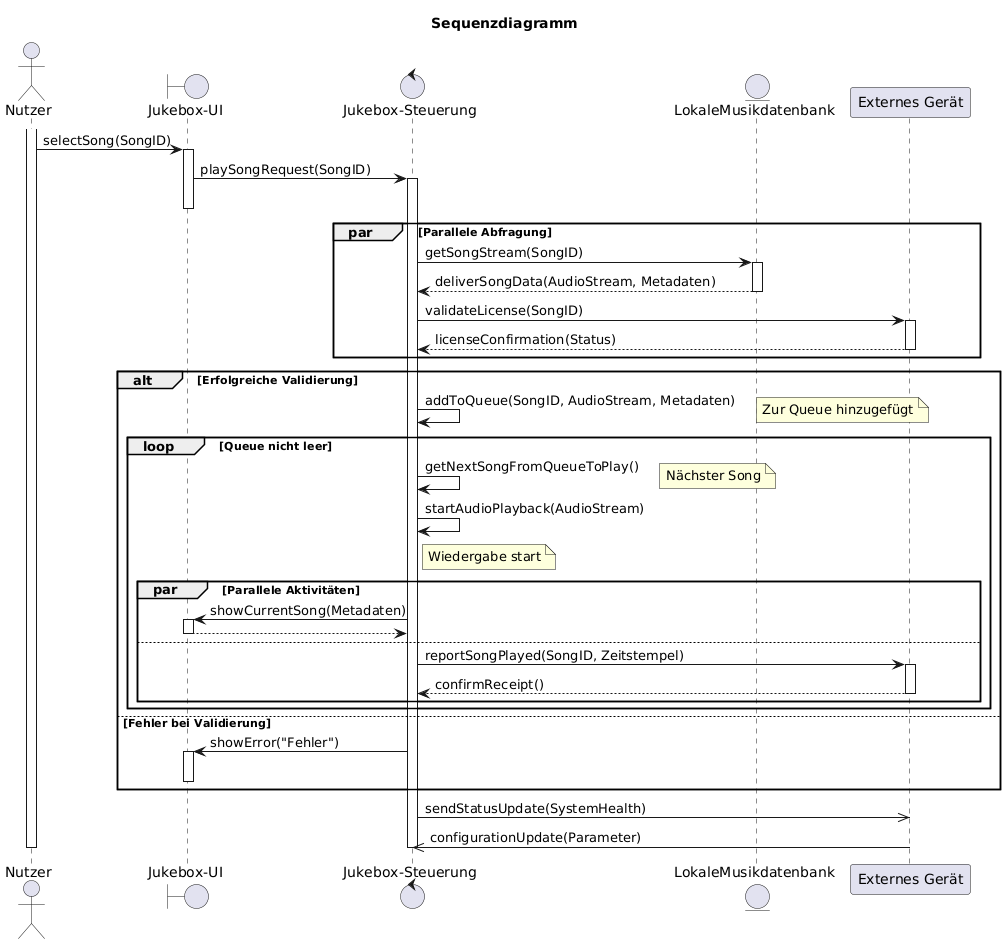
\includegraphics[width=\textwidth]{images/sequence_diagram.png}
    \caption{UML-Sequenzdiagramm: Zeitliche Abfolge der Komponenten-Interaktionen bei Songwiedergabe}
    \label{fig:sequence_diagram}
\end{figure}
\noindent
\textbf{Ablauf:}\\
Der Ablauf beginnt mit der Songauswahl (\texttt{selectSong()}) durch den Nutzer über die UI. Die Steuerung ruft parallel Audiodaten von der lokalen Datenbank ab und validiert die Lizenz über das externe Gerät (\texttt{validateLicense()}). Nach erfolgreicher Validierung startet die Wiedergabe (\texttt{startAudioPlayback()}) und die UI wird entsprechend aktualisiert. Abschließend wird die Wiedergabe protokolliert, während kontinuierliches Monitoring zwischen Steuerung und externem Gerät erfolgt.

\section{Fazit} \label{sec:fazit}

Die UML-basierte Spezifikation des Musikautomaten mittels Aktivitäts- und Sequenzdiagramm bietet unterschiedliche Perspektiven auf die Systemfunktionalität und ermöglicht eine strukturierte Analyse der komplexen Nutzer-System-Interaktion.

\subsection{Diagrammqualität und funktionale Abdeckung}

Das Aktivitätsdiagramm (\ref{fig:activity_diagram}) visualisiert den nutzerzentrierten Hauptprozess transparent durch Swimlanes und erfasst sowohl optimale Abläufe als auch wesentliche Verzweigungen. \\
Das Sequenzdiagramm (\ref{fig:sequence_diagram}) ergänzt dies durch detaillierte Darstellung zeitlicher Abhängigkeiten und Nachrichtenaustausche, insbesondere mit externen Systemen für Lizenzvalidierung und Compliance.\\
\textbf{Vollständig abgedeckte Aspekte:}
Kompletter Nutzungsworkflow, interaktive Songauswahl, Lizenzvalidierung, grundlegende Fehlerbehandlung, bidirektionale Kommunikation mit Überwachungsinfrastruktur und Echtzeit-Statusübermittlung.\\
\textbf{Teilweise abgedeckte Funktionalitäten:}
Erweiterte Fehlerbehandlung (Netzwerkausfälle, Hardwaredefekte) und Wartungsprozesse sind nur konzeptuell erfasst, was jedoch für die primär manuellen Offline-Tätigkeiten vertretbar ist.

\subsection{Methodische Limitationen}
Die gewählten Diagrammtypen decken die Kernfunktionalitäten umfassend ab, stoßen jedoch bei folgenden Aspekten an Grenzen:
\begin{itemize}
\item \textbf{Systemzustände:} Betriebsmodi und Transitionen wären durch Zustandsdiagramme präziser modellierbar
\item \textbf{Architektur:} Strukturelle Aspekte erfordern Komponenten- oder Verteilungsdiagramme
\item \textbf{Datenmodell:} Persistente Strukturen benötigen Klassendiagramme
\item \textbf{Nebenläufigkeit:} Parallele Prozesse sind in den gewählten Diagrammen nur eingeschränkt darstellbar
\end{itemize}
\noindent
Die Diagramme erfüllen ihren Zweck als prozess- und interaktionsorientierte Spezifikation, während strukturelle und zustandsbasierte Aspekte durch ergänzende UML-Diagrammtypen vollständiger erfasst werden könnten.

\end{document}